\documentclass[conference,10pt]{IEEEtran}
\IEEEoverridecommandlockouts
% The preceding line is only needed to identify funding in the first footnote. If that is unneeded, please comment it out.
\usepackage{cite}
\usepackage{amsmath,amssymb,amsfonts}
\usepackage{algorithm,algorithmic}
\usepackage{graphicx}
\usepackage{textcomp}
\usepackage{xcolor}
\usepackage{url}
\usepackage[hidelinks]{hyperref}
\usepackage{hhline}
\usepackage{verbatim}
\usepackage{array}
\def\BibTeX{{\rm B\kern-.05em{\sc i\kern-.025em b}\kern-.08em
   T\kern-.1667em\lower.7ex\hbox{E}\kern-.125emX}}
   
\begin{document}

\newcommand{\Fix}[1]{\textbf{[[#1]]}}
\newcommand{\Code}[1]{\begin{small}\texttt{#1}\end{small}}

% This two commands changes spacing between equations
\setlength{\belowdisplayskip}{2pt} \setlength{\belowdisplayshortskip}{2pt}
\setlength{\abovedisplayskip}{3pt} \setlength{\abovedisplayshortskip}{3pt}
 
% This command reduces spacing below single column figure and tables
\setlength{\textfloatsep}{0.6\baselineskip plus 0.2\baselineskip minus 0.2\baselineskip}

% This command reduces spacing above foot notes
\setlength{\skip\footins}{4pt}

% IMPORTANT: This paper MUST convey the following information
% 1. the envisioned users;
% 2. the software engineering challenge it proposes to address;
% 3. the methodology it implies for its users; and
% 4. the results of validation studies already conducted for mature tools, or the design of planned studies for early prototypes.

% IMPORTANT: ICSE Demonstration Track Evaluation Criteria
% 1. the relevance of the proposed demonstration for the ICSE audience;
% 2. the technical soundness of the submission;
% 3. the originality of its underlying ideas;
% 4. the quality of its presentation in the associated video; and
% 5. the degree to which it considers the relevant literature.

% IMPORTANT: 论文撰写中的一些约定
% 1. 对于论文内容的重要评论和TODO,使用\Fix命令,会在正文醒目标出
% 2. 对于论文内容的次要评论和提示,直接留下注释即可
% 3. 对于需要用等宽字体的场合,使用\Code命令

\title{MigrationAdvisor: Recommending Library Migrations from Large-Scale Open-Source Data}

\author{\IEEEauthorblockN{Hao He\IEEEauthorrefmark{1}, Yulin Xu\IEEEauthorrefmark{1}, Xiao Cheng\IEEEauthorrefmark{2}, Guangtai Liang\IEEEauthorrefmark{2}, and Minghui Zhou\IEEEauthorrefmark{1}\textsuperscript{\textsection}}
\IEEEauthorblockA{\IEEEauthorrefmark{1}Department of Computer Science and
Technology, Peking University, Beijing, China\\
\IEEEauthorrefmark{1}Key Laboratory of High Confidence Software Technologies, Ministry of Education, China\\
Software Analysis Lab, Huawei Technologies Co., Ltd., China\IEEEauthorrefmark{2}\\
Email: \{heh, kylinxyl, zhmh\}@pku.edu.cn\IEEEauthorrefmark{1},
\{chengxiao5, liangguangtai\}@huawei.com\IEEEauthorrefmark{2}
}}

\maketitle

\begingroup\renewcommand\thefootnote{\textsection}
\footnotetext{corresponding author.}
\endgroup

\begin{abstract}
During software maintenance, developers may need to migrate an already in-use library to another library with similar functionalities.
However, it is difficult to make the optimal migration decision with limited information, knowledge, or expertise. 
In this paper, we present \textsc{MigrationAdvisor}, an evidence-based tool to recommend library migration targets through intelligent analysis upon a large number of GitHub repositories and Java libraries. 
The migration advisories are provided through a search engine style web service where developers can seek migration suggestions for a specific library.
We conduct systematic evaluations on the correctness of results, and evaluate the usefulness of the tool by collecting usage feedback from industry developers.
Video:  \url{https://youtu.be/4I75W22TqwQ}.
\end{abstract}

\begin{IEEEkeywords}
library migration, mining software repositories, library recommendation, dependency management
\end{IEEEkeywords}

\section{Introduction}

The wide adoption of open-source third-party libraries in modern software systems is beneficial but also risky. 
Third-party libraries may be abandoned by their maintainers, may have license incompatibilities, or may fail to satisfy new requirements due to absence of features, low performance, etc.
To address these issues, developers need to migrate an already in-use library (i.e., \textit{source library}) to another similar or functionality equivalent library (i.e., \textit{target library}) for their software projects. Such activities are called as \textit{library migration} in the related literature~\cite{teyton2012mining, teyton2014study, kabinna2016logging, alrubaye2019migrationminer}.

However, it is often non-trivial to find target libraries and choose the best target library for a software project. 
Existing library comparison information on the Internet (e.g., blog posts, forum discussions, community curated lists) are mostly opinion-based, likely outdated, and inherently controversial.
Existing works on distilling library differences~\cite{2020FSE-DiffTech} and mining similar libraries~\cite{chen2016similartech} may help quickly locate a set of possible target libraries, but the former is still summarizing opinions and the latter provides no evidence on the feasibility of a migration.
In practice, software projects rely heavily on core developers for making the migration decision, but the decision may be sub-optimal, especially when developers have limited knowledge or experience with the candidate target libraries.

To address this situation, several approaches have been proposed to mine existing library migrations from a large corpus of software repositories~\cite{teyton2012mining, teyton2014study, alrubaye2019migrationminer}.
The underlying rationale is that historical migration practices provide valuable reference and guidance for developers when they make migration decisions.
However, the existing works suffer from either low performance or limited scale which limits their usefulness in practice (More details in Section~\ref{sec:related-work}).

In this paper, we present \textsc{MigrationAdvisor}, an accurate and evidence-supported library migration recommendation tool to support decision making before conducting a library migration in a Java project.
Our tool works upon an advisory database built from a large corpus of Java GitHub repositories and Maven artifacts. 
Given a source library that a user wants to migrate for his/her project, it will generate a set of candidate target libraries from the repositories, compute a set of metrics for each candidate, and rank them using a combined confidence value. 
Finally, the ranked candidate targets and the possible migration commits for each target will be returned for human inspection.
We expect our tool to be used by project maintainers to seek migration suggestions for a library they are already using, evaluate between a set of candidate target libraries, or support their migration decisions for a specific target library. 
We also plan to integrate our tool in an enterprise-level library management process which aims to support and secure third-party library usage in IT companies.

We systematically evaluate the correctness of recommendation results in a technical paper~\cite{our-paper}, showing that our tool can recommend migration target libraries with MRR of 0.8566, top-1 precision of 0.7947, top-10 NDCG of 0.7702, and top-20 recall of 0.8939.
We further invite several industry developers to search libraries they know using our tool, and their feedback shows that the tool returns valid recommendations with useful evidences.
They also provide interesting comments and insights for future research.

Our tool is available at \url{http://migration-helper.net/}. 
The source code, data, evaluation scripts, and a RESTful backend is available at \url{https://github.com/hehao98/MigrationHelper}. The source code for frontend is available at \url{https://github.com/hehao98/MigrationHelperFrontend}.

\section{MigrationAdvisor Workflow}

\begin{figure*}[tb]
  \centering
  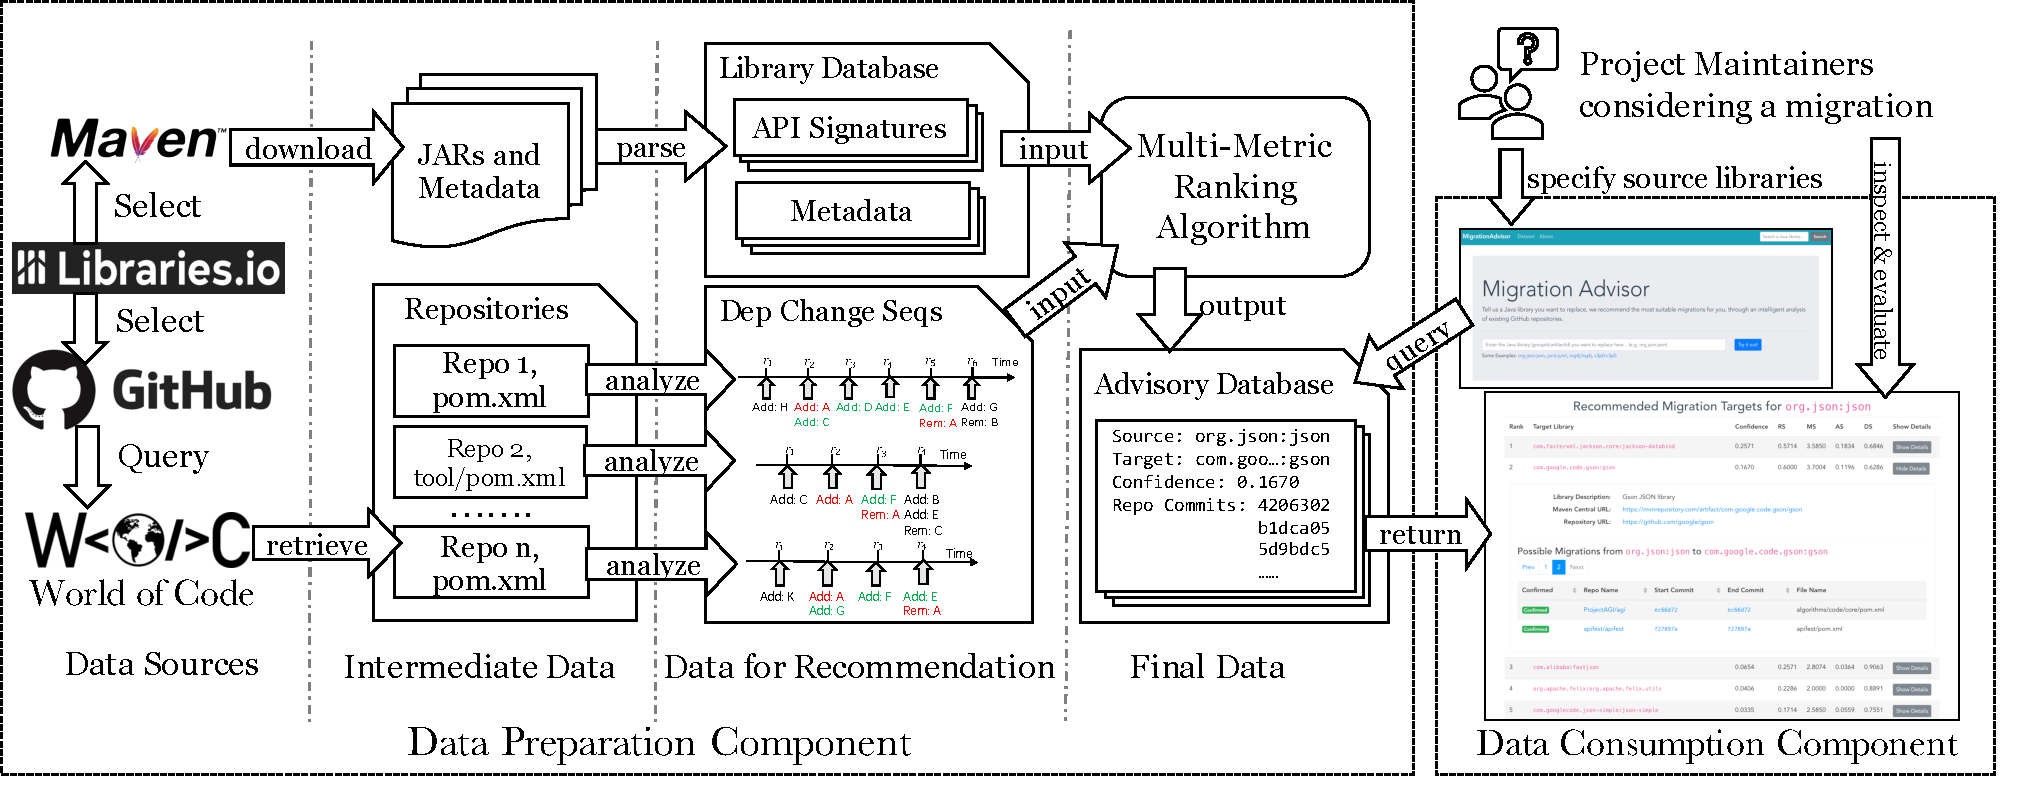
\includegraphics[width=0.92\textwidth]{fig/ToolDemo.pdf}
  \caption{Overview of \textsc{MigrationAdvisor}, with two major components. The data preparation component aggregates library and repository data for generating the advisory database. The data consumption component is an interactive frontend where developers can search for migration advisories given a specific library.}
  \label{fig:overview}
  \vspace{-5mm}
\end{figure*}

Figure~\ref{fig:overview} provides an overview of \textsc{MigrationAdvisor}. 
It has two major components: a data preparation component and a data consumption component.
The data preparation component aggregates and processes repository and library data from multiple sources, runs a recommendation algorithm for all libraries in the collected data, and stores the results in an advisory database. 
The data consumption component serves user requests when they seek migration advice for some given source libraries. Given a source library, it will query the advisory database and return a set of target libraries so that the users can inspect and evaluate different migration targets.

\subsection{Data Preparation}

Given an ecosystem we want to support, the data preparation component (Figure~\ref{fig:overview}, left) aims to collect necessary information, evidence and existing migrations from the development histories of open-source projects.
We choose to implement our tool for Java and Maven because of their popularity and industry importance.
We use latest Libraries.io dataset~\cite{libraries-io} (last updated January 2020) for selecting libraries and repositories of interest, where we get a list of 184,817 distinct libraries (i.e. Maven artifacts with distinct group ID and artifact ID) and a list of 21,358 Maven managed non-fork GitHub repositories with at least 10 stars and three \Code{pom.xml} changes. %%10以下用单词

For each library, we retrieve its version information and other metadata from Maven Central, resulting in 4,045,748 distinct library versions.
For each version, we download its corresponding JAR file from Maven Central, if it has one, and extract all public classes from the JAR file. 
For each class, it is transformed into a compact API signature document which encodes all its public fields, methods, and inheritance relationships.
The documents are stored in a library database.
% The total size of downloaded JARs is $\sim$3TB, but they can be safely deleted after the parsing is finished.
Other library metadata (e.g. versions, dependencies and descriptions) are also stored in the library database for further use.

For each GitHub repository, we retrieve all its version control data (i.e. commits, trees, blobs) from the World of Code database~\cite{ma2019world} (version R, last updated in April 2020), which includes all GitHub repositories mentioned before.
We use World of Code because it offers much higher performance for analytical purposes, compared with directly cloning from GitHub and analyzing with \Code{git}.
We then collect all \Code{pom.xml} files and all their historical versions in this repository. %\footnote{In a Maven managed project, a \texttt{pom.xml} file declares all the libraries it uses in the \texttt{<dependency>} section. A repository may have more than one \texttt{pom.xml} files in different paths, which are used to manage dependencies of different sub-modules or sub-projects.}.
For each \Code{pom.xml} file, we iterate over all its historical versions and compare with its previous version, to extract the dependency changes happened in this version.
By merging dependency changes from different commits and branches, we generate a dependency change sequence for each \Code{pom.xml} file, which contains all library adoption, removal and update histories for this \Code{pom.xml} file.
% Finally, all the sequences, along with other repository version control data, are stored in a database for further use.

Given the data described above, the final migration advisory database is generated by a multi-metric ranking algorithm for migration target recommendation.
For each library we collect, the algorithm first generates a set of candidate target libraries by analyzing the dependency change sequences.
Then, it computes several metrics for each candidate: Rule Support ($RS$), Message Support ($MS$), API Support ($AS$) and Distance Support ($DS$). The metrics are intended to identify real target libraries from the large number of false positives in the initial set of candidates, by capturing different dimensions of evidences from the collected data.
More specifically, $RS$ captures frequently added and removed libraries in the same commit; $MS$ captures libraries that developers stated a migration in the commit messages; $AS$ captures frequent code changes between the method calls of two libraries; and $DS$ captures hints from commit topology. 
After that, it computes confidence value from all metrics using a simple multiplication
\begin{equation}
    confidence(lib_A, lib_B) = RS \cdot MS \cdot AS \cdot DS
\end{equation}
which represents the likelihood that the candidate library is an eligible migration target for the source library. 
% Finally, we store all source/target library pairs,  metrics, confidence values, and related GitHub commits in the advisory database. 
The algorithm is detailed in a technical paper~\cite{our-paper}.

To enhance user experience, we also mark a subset of ground truth migration advisories in the advisory database. 
The ground truth comes from a systematic labelling process detailed in~\cite{our-paper}, including source/target library pairs, migration commits, and related \Code{pom.xml} changes. 
The ground truth migration advisories can also be extended and curated in a crowd-sourced manner when more users use our tool.

Table~\ref{tab:db} shows the statistics of the data used in current tool implementation. The data can be periodically updated to reflect latest trends in the open-source community.

\begin{table}[t]
\caption{Statistics of the database used in our tool. API Count is an intermediate data table used during metric computation.
}
\centering
\begin{tabular}{|l|r|l|}
\hline
\textbf{Data Type} & \textbf{Count or Size} & \textbf{Time to Construct}  \\ \hhline{|=|=|=|}
GitHub repositories        & 21,358 & Several minutes   \\ \hline
Commits with diffs         & 29,439,998  & About 1 day  \\ \hline
Parsed \texttt{pom.xml}s   & 10,009,952  & About 1 day  \\ \hline
Dep change seqs            & 147,220  & Several hours \\ \hline
Libraries                  & 185,817  & Several minutes  \\ \hline
Library versions           & 4,045,748  & Several hours  \\ \hline
Java classes               & 25,272,024  & About 3 days  \\ \hline
Non-zero API counts        & 4,934,677 & About 2 weeks     \\ \hline
Migration advisories       & 1,956,809 & Several hours     \\ \hline
Ground truth advisories    & 14,334    & 1 week (manually) \\ \hline
Database size (gzip dump)  & $\sim$50GB & Several weeks     \\ \hline
\end{tabular}
\label{tab:db}
\end{table}

\subsection{Data Consumption}

The data consumption component (Figure~\ref{fig:overview}, right) serves as an interface to project developers and maintainers.
Given a source library to be migrated, it should provide informative and interactive demonstrations of the migration recommendations from the advisory database.
For current tool demo, it is implemented as a search engine style web service, where users can search for the migration targets of a specific library.
Given a search query, the web service will retrieve all target libraries from the advisory database, sort them by the confidence value, and return them in a paginated table where each table entry demonstrates one target library.
For each entry, users can also extend the entry for more detailed information, including library description, homepage, repository links, and GitHub repositories/commits that may have performed a migration from the given source library to the target library in this entry. 
Interested users can click on the links to browse more information about the target library and the migration commits.

\section{Implementation}\label{s:implementation}

% The tool is implemented as a web service that comprises two components.

The data preparation component is implemented using a combination of Java programs and Python scripts, where each program or script implements one data processing stage (i.e. an arrow) in Figure~\ref{fig:overview}.
All programs and scripts are executed on one of the World of Code~\cite{ma2019world} server nodes, which is a Red Hat Linux server with 2 Intel Xeon E5-2630 v2 CPUs, 400GB RAM and 20TB storage. 
The total size of intermediate data (i.e., library JARs and raw git objects) exceeds 4 TB, but they are not needed for the data consumption component and can be safely deleted once the analysis is finished.
The library APIs, library metadata, repository metadata, dependency change sequences, the final migration advisories, and other relevant data are stored in a local MongoDB instance (See Table~\ref{tab:db} for its statistics).
The data consumption component only needs to read from this database, so it is relatively lightweight and has flexible deployment options.
% Currently, it is implemented as a demo web service, in which the backend is a RESTful Spring Boot application, and the frontend is a progressive web application built with Vue.js and Bootstrap.
Currently, the frontend, backend, and a MongoDB instance are hosted on an AWS virtual Linux server with 2 CPU cores, 8GB RAM, and 200GB storage. 

\section{Tool Usage}

We expect \textsc{MigrationAdvisor} to be used when project maintainers discover that one of the libraries in their project need to be replaced (due to license, security, internal industry standards, etc).
Suppose a developer wants to migrate from \Code{org.json:json} because its license is incompatible with Apache 2.0 license.
Using our web service, she can type \Code{org.json:json} in the search input and click the ``Search'' button, as shown by the web page on the right part of Fig~\ref{fig:overview}.
Then the service will return a list of recommended migration targets, the top-3 being \Code{jackson}, \Code{gson} and \Code{fastjson}.
She can immediately discover that \Code{jackson} seems to be a good choice because most projects migrate to \Code{jackson} and it is also licensed under Apache 2.0.
If she is more prudent, she can carefully investigate the migration commits and even combine our tool with other approaches to make the final decision.

In the future, we plan to integrate this component with existing third-party library checking software, either as an IDE plugin or as part of a CI/CD process.
When the checking software identifies incompatible, deprecated, or banned libraries, our tool will prompt migration advisories to help developers quickly locate a target library that they can migrate to.

\section{Evaluation}

Two aspects of \textsc{MigrationAdvisor} are evaluated. %should be evaluated. 
The first aspect is the correctness and completeness of migration advisories (i.e. whether the returned results are real migration targets and whether all migration targets are returned). 
The second aspect is to what extent this tool is helpful for developers when they make migration decisions.
%In this paper, we report the evaluation results of the first aspect %%%(more details in the technical paper~\cite{our-paper}) and %a preliminary evaluation plan for the second aspect.
%and developer trial experiences for the second aspect.

For the first aspect, we use the following common performance metrics for evaluating information retrieval and ranking problems: Mean Reciprocal Rank (MRR),
%~\cite{Craswell2009MRR}, 
top-$k$ precision, top-$k$ recall and top-$k$ Normalized Discounted Cumulative Gain (NDCG).
%~\cite{2002-NDCG}. 
% The performance are computed on a set of ground truth 
% that we recover from an existing work~\cite{teyton2014study} and systematically extend in latest GitHub repositories. 
Table~\ref{tab:perf-comp} shows the results of the algorithm used in our tool and the results of two existing approaches~\cite{teyton2012mining, alrubaye2019migrationminer} on the ground truth advisories.
We can see from Table~\ref{tab:perf-comp} that the multi-metric ranking algorithm significantly outperforms existing work, reaching MRR of 0.8566, top-1 precision of 0.7947, top-10 NDCG of 0.7702, and top-20 recall of 0.8939.
% To the best of our knowledge, we achieve the best overall performance in this problem domain.
% (Note that the the approach in Alrubaye et al.~\cite{alrubaye2019migrationminer} has higher top-1 precision but its recall is significantly lower). 
% Therefore, we conclude to the best of our knowledge that our algorithm achieves best overall performance, and our tool can provide the most accurate and complete migration advisories.

\begin{table}[t]
\caption{Performance of the multi-metric ranking algorithm used in MigrationAdvisor, compared with other existing approaches.}
\centering
\begin{tabular}{|l|r|r|r|r|}
\hline
\textbf{Approach} & \textbf{MRR} & \textbf{Precision@1} & \textbf{NDCG@10} & \textbf{Recall@20}  \\ 
\hhline{|=|=|=|=|=|}
Teyton et al.             & 0.7335 & 0.6757 & 0.6909 & 0.6391 \\ \hline
Alrubaye et al.           & 0.9412 & 0.9412 & 0.9412 & 0.0540 \\ \hline
Our Approach              & 0.8566 & 0.7947 & 0.7702 & 0.8939 \\ \hline
\end{tabular}
\label{tab:perf-comp}
\end{table}

For the second aspect, we invite industry developers in our social network\footnote{This is done by sharing posts in a number of group chats ($\sim$100 people in total), but it is hard to count the exact number of developers reached.} to search libraries they know using our tool, and collect their usage feedback through informal communications. 
They provide positive feedback and interesting insights about our tool.
One developer replies that \textit{finding replaceable and actively maintained software is what we really need for legacy software}.
%Another developer suggests that our tool should also issue a warning if no substitute library is available.
They also suggest that our tool should return reasons for each recommendation, and issue warnings when no migration target is available.
However, we also discover that only a small fraction of developers have experience on library migrations, and one reason may be that most developers we contact are in relatively junior positions and have limited years of working experience, but it should be explored in future research.
By monitoring our website in a two-month period, we record search attempts from 68 different IPs. Figure~\ref{fig:usage} shows user geographic information and most frequently searched libraries.
% 48 search attempts from 27 different IPs are recorded and we receive responses from five developers who work in software engineering tool, cloud computing or security teams.
% They try different libraries (e.g. \Code{dom4j}, \Code{guava}, \Code{hbase}, \Code{antlr}, etc) and generally think that our tool can return valid recommendation results with useful evidences.
% We are also advertising our tool, running online questionnaires and monitoring the usage statistics of our website for a systematic validation study in the future.

\begin{figure}[tb]
  \centering
  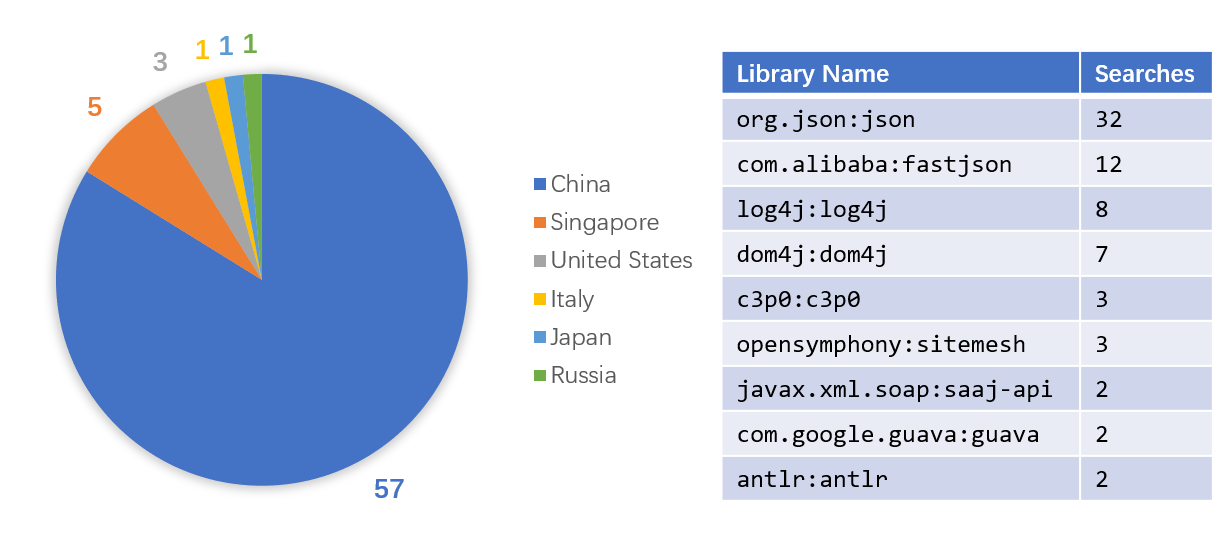
\includegraphics[width=0.4\textwidth]{fig/Usage.png}
  \vspace{-4mm}%%%%zhmh: how many developers provided feedback? the number could be provided.
  \caption{User geographic information and most frequently searched libraries}
  \label{fig:usage}
  \vspace{-1mm}
\end{figure}

\section{Related Work}
\label{sec:related-work}

Several existing tools and websites also aims to help developer select between libraries or conduct library migrations, but they all have limitations in this problem context.
%in the context of migration target recommendation.
% APIWave~\cite{hora2015apiwave} tracks API popularity and migrations of 650 popular Java GitHub repositories, but its scale is limited and the most popular API changes in code may not be useful enough for developers seeking migration suggestions.
SimilarTech~\cite{chen2016similartech} recommends similar libraries through Stack Overflow tag embeddings, but it provide no evidence on the feasibility of migrations between the query library and returned libraries.
LibComp~\cite{2020FSE-LibComp} is a metric-based comparison tool for similar libraries, but it requires manual specification of two libraries and cannot help developers when they are unaware of a possible migration target.
There are also community efforts such as AlternativeTo\footnote{\url{https://alternativeto.net/}},
%~\cite{alternative-to}
a crowd-sourced software recommendation website, and \Code{awesome-java}\footnote{\url{https://github.com/akullpp/awesome-java}},
%~\cite{awesome-java}
a community curated Java library list organized into many categories.
Library comparison blog posts and forum discussions\footnote{Unfortunately, the well-known Stack Overflow does not allow opinion-based discussions including the topic of library comparison and selection (See \url{https://meta.stackoverflow.com/questions/255468/opinion-based-questions}).
%~\cite{stack-overflow-opinion}
} can be accessed using a search engine, and DiffTech~\cite{2020FSE-DiffTech} can be used to aggregate community opinions of similar libraries from online discussions.
However, these approaches can only return opinion-based results which are inherently controversial and may not be trust-worthy.
Despite their limitations, our tool is not intended to fully replace any of the existing approaches, 
but to \textit{enhance} migration decision making through providing objective evidence of historical migration practices. 
Developers can refer to our tool and any existing approaches above to make the optimal decision for his/her project.

Some existing approaches share the same objective as our tool, but they suffer from performance issues which limit their usefulness in practice.
Teyton et al.~\cite{teyton2012mining} propose a filtering-based approach on mining library migrations, but it suffers from either low precision or low recall depending on the filtering threshold.
MigrationMiner~\cite{alrubaye2019migrationminer} uses a different filtering-based approach, but it is only evaluated on 16 GitHub repositories (by contrast, 21,358 analyzed in our tool). 
To the best of our knowledge, our tool is the first accurate, large-scale, and evidence-supported library migration recommendation tool being able to recommend migration target libraries based on large-scale open-source data.

Other tools aim to support library migrations by providing API mappings (e.g. SimilarAPI~\cite{chen2020similarapi}) or directly transform code to use the new library (e.g. Meditor~\cite{xu2019meditor}). 
Developers can use the results of our tool as the input to these tools, to improve development efficiency during library migrations.

\section{Conclusion}

We present \textsc{MigrationAdvisor}, an evidence-supported library migration recommendation tool which works upon a migration advisory database built from a large corpus of GitHub repositories and Java libraries.
In the future, we plan to improve our tool from various perspectives, such as reason extraction, cost estimation, and customized recommendation.
% In the future, we plan to improve our tool based on the feedback we collected. 
% We also plan to develop new techniques to summarize reasons for a migration and estimate migration costs, to make our tool more useful.

\section*{Acknowledgment}

This work is supported by the National Key R\&D Program of China Grant 2018YFB1004201, the National Natural Science Foundation of China Grant 61825201, and the Open Fund of Science and Technology on Parallel and Distributed Processing Laboratory (PDL) No.6142110810403.

\bibliography{ref.bib}
\bibliographystyle{IEEEtran}

\end{document}
